% $Header: /cvsroot/latex-beamer/latex-beamer/solutions/generic-talks/generic-ornate-15min-45min.en.tex,v 1.4 2004/10/07 20:53:08 tantau Exp $

\documentclass{beamer}

% This file is a solution template for:

% - Giving a talk on some subject.
% - The talk is between 15min and 45min long.
% - Style is ornate.



% Copyright 2004 by Till Tantau <tantau@users.sourceforge.net>.
%
% In principle, this file can be redistributed and/or modified under
% the terms of the GNU Public License, version 2.
%
% However, this file is supposed to be a template to be modified
% for your own needs. For this reason, if you use this file as a
% template and not specifically distribute it as part of a another
% package/program, I grant the extra permission to freely copy and
% modify this file as you see fit and even to delete this copyright
% notice. 


\mode<presentation>
{
  \usetheme{Warsaw}
  % or ...

  \setbeamercovered{transparent}
  % or whatever (possibly just delete it)
}


\usepackage[english]{babel}
% or whatever

\usepackage[latin1]{inputenc}
% or whatever

\usepackage{times}
\usepackage[T1]{fontenc}
% Or whatever. Note that the encoding and the font should match. If T1
% does not look nice, try deleting the line with the fontenc.

\usepackage{multimedia}

\title[Negotiating the musical work.] % (optional, use only with long paper titles)
{Negotiating the musical work.}

\subtitle
{An empirical study.}

\author[Frisk, \"{O}stersj\"{o}] % (optional, use only with lots of
				 % authors)
{Henrik Frisk \and Stefan �stersj�}
%{Henrik Frisk \and Stefan
%\"{O}stersj\"{o}\\ \texttt{henrik.frisk@mhm.lu.se}, \texttt{stefan_ostersjo@hotmail.com}}
% - Use the \inst{?} command only if the authors have different
%   affiliation.

\institute[Malm\"{o} Academy of Music, Lund University] % (optional, but mostly needed)
{
  Malm\"{o} Academy of Music\\
  Lund University
}
% - Use the \inst command only if there are several affiliations.
% - Keep it simple, no one is interested in your street address.

\date[ICMC-06] % (optional)
{ICMC 2006}

\subject{Talks}
% This is only inserted into the PDF information catalog. Can be left
% out. 

% If you have a file called "university-logo-filename.xxx", where xxx
% is a graphic format that can be processed by latex or pdflatex,
% resp., then you can add a logo as follows:

 \pgfdeclareimage[height=1cm]{university-logo}{Ulomacvpmse}
 \logo{\pgfuseimage{university-logo}}



% Delete this, if you do not want the table of contents to pop up at
% the beginning of each subsection:
%\AtBeginSubsection[]
%{
%  \begin{frame}<beamer>
%    \frametitle{Outline}
%    \tableofcontents[currentsection,currentsubsection]
%  \end{frame}
%}


% If you wish to uncover everything in a step-wise fashion, uncomment
% the following command: 

\beamerdefaultoverlayspecification{<+->}


\begin{document}

\begin{frame}
  \titlepage
\end{frame}

\begin{frame}
  \frametitle{Outline}
  \tableofcontents[pausesections]
\end{frame}


% Since this a solution template for a generic talk, very little can
% be said about how it should be structured. However, the talk length
% of between 15min and 45min and the theme suggest that you stick to
% the following rules:  

% - Exactly two or three sections (other than the summary).
% - At *most* three subsections per section.
% - Talk about 30s to 2min per frame. So there should be between about
%   15 and 30 frames, all told.

\section{Introduction}

\subsection[Purpose]{Conditions, Purpose and Terminology}

\begin{frame}
  \frametitle{Conditions, Purpose and Terminology}
  % - A title should summarize the slide in an understandable fashion
  %   for anyone how does not follow everything on the slide itself.

  \begin{itemize}
   \item
	The musical work before its ultimate notation and performance.
   \item
	Mixed media music - music for instruments and (live) electronics.
   \item 
	Wish to gain a deeper understanding of the underlying processes in the
	communication between the composer and the performer.
   \item 
	Making use of this knowledge when working on
	interactive performance systems.
  \end{itemize}
\end{frame}

\subsection[Music - Notation]{Music and Notation}

\begin{frame}
  \frametitle{Music and notation and the two agents.}

 \includegraphics<1>[height=3.5cm]{img/cons-rep2.pdf}
 \pause
 \includegraphics<2>[height=3.5cm]{img/cons-rep-ric2.pdf}
 \pause
 \includegraphics<3>[height=3.5cm]{img/cons-rep-rep-cons2.pdf}
\end{frame}

\section{Method}
\subsection[Musical Semiology]{Semiological approach}

\begin{frame}
 \frametitle{Musical Semiology}
 \begin{itemize}
  \item {Analytical understanding of the musical work in its entirety.}
  \item {{\itshape The notion of a 'single, well-defined item of
	information to be transmitted, all the rest being simply noise'
	is 'misleading as soon as we move
	from the artificial communication of information to a concrete
	act of human communication [...]' }(Molino)}
  \item {{\itshape '...recognizing, elaborating, and articulating the
	three relatively autonomous levels (poietic, neutral and
	esthesic) facilitates knowledge of all processes unleashed by
	the musical work [...]' }(Nattiez)}
 \end{itemize}
\end{frame}

\begin{frame}
  \frametitle{The Three Autonomous Levels.}

 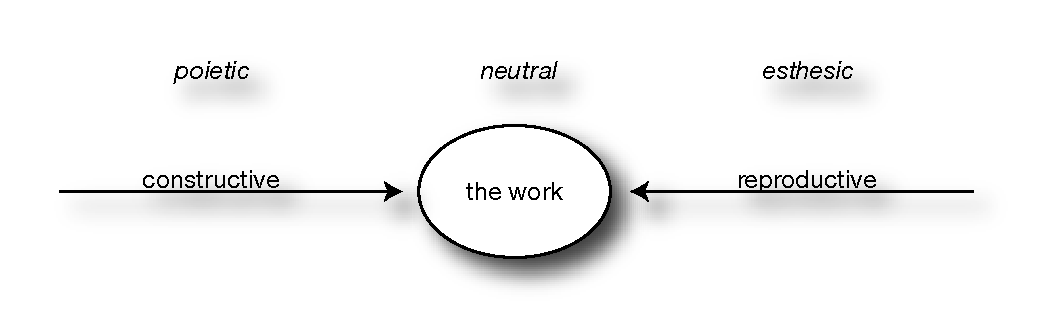
\includegraphics[height=3.5cm]{img/cons-rep-semiology.pdf}
 \begin{itemize}
  \item{the poietic - the constructive phase}
  \item{the esthesic - the interpretative phase}
  \item{the neutral - the trace}
 \end{itemize}
\end{frame}

\begin{frame}
 \frametitle{Method - Summary}
\begin{itemize}
 \item Drawing on Nattiez and Molino and their idea of tripartition.
 \item Using a qualitative method for the selection of material for
       analysis.
 \item Doing a verbatim transcription of video documentation from which a graph
       was extracted. 
 \item For an indepth review of the method and theory for this study,
       see http://www.ems-network.org.
\end{itemize}
\end{frame}

\section{Empirical Studies}

\subsection[Harp]{Excerpts from harp piece}
\begin{frame}
  \frametitle{Four notations of the same two bars.}

 \includegraphics<1>[height=2.5cm]{img/score/eps/harpVersion1.pdf}
 \pause
 \includegraphics<2>[height=3.5cm]{img/score/eps/harpVersion2.pdf}
 \pause
 \includegraphics<3>[height=3.5cm]{img/score/eps/harpVersion3.pdf}
 \pause
 \includegraphics<4>[height=4cm]{img/score/eps/harpVersion4.pdf}
\end{frame}

\begin{frame}
\frametitle{Conclusions}
\begin{itemize}
 \item Negotiations between the 'vision' and the idiomatic constraints
       of the instrument.
 \item The presence of the performer led to new impulses.
 \item Poietic analysis: music \alert{was not} altered.
 \item Neutral analysis: music \alert{was} altered.
 \item Shows the recursive nature of the interplay between poietic and
       esthesic processes.
\end{itemize}
\end{frame}

\subsection[Viken]{Love Mangs' Viken}

\begin{frame}
 \frametitle{Explicit intentions of the collaboration}
\begin{itemize}
 \item A piece that uses real-time sound processing.
 \item Investigate the boundaries between composing and performing.
 \item Use of improvisation.
 \item Purpose of the documented session: To work out variations on the
       melody...
\end{itemize}
\end{frame}

\begin{frame}
 \frametitle{Notation of the excerpt.}
 \includegraphics<1->[width=0.9\textwidth]{img/viken.pdf}\\
 \pause
 \includegraphics<2->[width=0.9\textwidth]{img/score/viken8b.pdf}
 \movie[externalviewer]{snd}{img/embryo.mp3}
\end{frame}

\begin{frame}
\frametitle{First video clip - transcription / graph}
 \includegraphics<1>[width=0.75\textwidth]{img/transcription1.pdf}
 \pause
 \includegraphics<2>[width=0.75\textwidth]{img/timeline-section1.pdf}
\end{frame}

\begin{frame}
\movie[externalviewer]{play movie}{img/clips/Sequence1.mov}\\
\movie[externalviewer]{play movie with transcript}{img/clips/Sequence1-grph-trnscrpt.mov}\\
\end{frame}

\begin{frame}
\frametitle{The complete graph.}
 \includegraphics<1>[width=0.3\textwidth]{img/timeline_horiz.pdf}
\pause
 \includegraphics<2>[width=0.6\textwidth]{img/timeline-section2.pdf}
\end{frame}


\section{Discussion}

\subsection[Whose work?]{Whose work? Whose performance?}

\begin{frame}
\frametitle{Whose work and whose performance?}
\begin{itemize}
 \item Are the roles swapped? The roles of composer and performer seem
       to overlap.
 \item Composition may be regarded as a complex interaction between
       esthesic and poietic processes.
 \item Performers may similarly be said to oscillate between these two
       modes of artistic activity.
 \item The work may be seen as the result of a collaboration between
       multiple agents.
\end{itemize}
\end{frame}

\subsection[Interactivity]{Interactivity}

\begin{frame}
\frametitle{Interactivity between the two agents.}
\begin{itemize}
 \item Remarkable flexibility in the communication.
 \item Complete misunderstandings lead to the inclusion of new material.
 \item Noise in the communication - creative misunderstanding.
 \item A striking lack of synchronicity between the agents.
 \item An independent flow of the initiative, constructive and
       interpretative actions.
\end{itemize}
\end{frame}

\begin{frame}
\frametitle{Interactivity between a performer and a computer}
\pause
 Concepts we will attempt to use:
\begin{itemize}
 \item Noise in the communication may not be a problem.
 \item Direction may be more important than synchronicity.
 \item The initiative may shift \emph{independently} of the esthesic and
       poietic processes.
\end{itemize}
\end{frame}

\section*{Summary}

\begin{frame}
  \frametitle<presentation>{Summary}

  % Keep the summary *very short*.
  \begin{itemize}
  \item
       Composition and interpretation are activities that overlap to a
       significant degree.
  \item Analyzing these processes may alter the way we think of
       musician/machine interaction.
  \end{itemize}
  
  % The following outlook is optional.
  \vskip0pt plus.5fill
  \begin{itemize}
  \item
       Future work
       \begin{itemize}
	\item
	     Using the knowledge gained from these studies in a new
	     piece for 10-stringed guitar and computer.
	\item
	     Expanding the study to include more cases.
       \end{itemize}
  \end{itemize}
\end{frame}

\end{document}


